\chapter{Application des méthodes au problème}

	Dans cette partie, nous allons présenter comment les diverses techniques que nous souhaitons appliquer sont compatibles avec notre cas spécifique du sudoku.
    \section{A*}
    \section{Algorithme génétique}
    \section{Eco-résolution}
    Dans le chapitre, présentation des différents modèles nous avons présentés les divers attributs des eco-agents ainsi que leurs principales fonctions. \\
    L'éco-résolution est un mode de résolution utilisant plusieurs agents, la partie la plus complexe étant de définir quels sont nos agents et comment ils agissent entre eux. \\
    Nous avons ainsi défini le diagramme de classe suivant : \\
    \begin{center}
    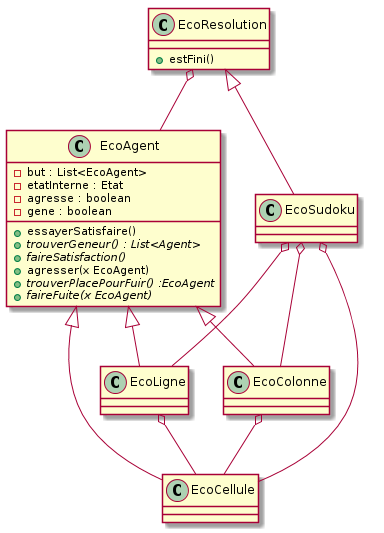
\includegraphics[scale=0.7]{diagrams/ecoResolution.png}
    \end{center} 

	Pour l'éco-résolution, nous retrouvons une seule méthode estFini(), qui vérifie lorsque tous les éco-agents de notre système sont satisfaits. \\
	Avant de démarrer l'éco-résolution, nous allons compléter les cases vides de notre sudoku. Les cases étant déjà dans l'énoncé comporteront un attribut cellType valant "GIVEN". Pour remplir notre sudoku, nous allons effectué un remplissage "intelligent", c'est-à-dire que dans chaque bloc nous allons placer une et une seule fois chaque numéro de 1 à 9.\\
	Nous avons choisi que nos cellules, nos lignes et nos colonnes seraient considérés comme éco-agent. \\
	
	\subsection{Les lignes}
	Nous allons voir les lignes comme éco-agent de la manière suivante : \\
	\begin{itemize}
	\item Le but d'une ligne est que tous les éco-agents qui la compose (cellule) aient des numéros différents.
	\item Pour trouver les gêneurs, cela correspondra à toutes les cellules qui ont un numéro qui intervient plus d'une fois. 
	\item FaireSatisfaction : Passer l'état comme étant satisfait
	\item une ligne ne pourra ni fuir, ni être en recherche de fuite.   
	\end{itemize}
	
	\subsection{Les colonnes}
	Nous allons voir les colonnes comme éco-agent de la manière suivante, analogue à la façon dont nous voyons les lignes : \\
	\begin{itemize}
	\item Le but d'une colonne est que tous les éco-agents qui la compose (cellule) aient des numéros différents.
	\item Pour trouver les gêneurs, cela correspondra à toutes les cellules qui ont un numéro qui intervient plus d'une fois. 
	\item FaireSatisfaction : Passer l'état comme étant satisfait
	\item une colonne ne pourra ni fuir, ni être en recherche de fuite.   
	\end{itemize}
	
	\subsection{Les cellules}
	Nous allons voir les cellules comme des agents de la manière suivante : 
	\begin{itemize}
	\item Une cellule est satisfaite si sa ligne et sa colonne sont satisfaites
	\item Les gêneurs d'une cellule sont les numéros ayant la même valeur sur la colonne et la ligne
	\item Pour FaireSatisfaction d'une cellule, il faut qu'il n'y ai plus de gêneur
	\item Pour trouverPlacePourFuir d'une cellule nous avons plusieurs idées : choisir une cellule aléatoirement dans le même bloc, choisir une cellule aléatoirement dans le bloc mais qui ne soit pas sur la ligne ou colonne de notre agent qui lance l'agression et enfin choisir la cellule qui a le plus de gêne.
	\item Pour faireFuite, nous allons échanger les numéros de nos deux cellules.
	\end{itemize}
